\documentclass[12pt,answers]{exam}

\usepackage[left=0.9in,right=0.9in,top=0.8in,bottom=1.05in]{geometry}
\newcommand{\ligne}[1]{\rule[0.5ex]{\textwidth}{#1}\\}

\usepackage[]{graphicx}
\usepackage{wrapfig}
\usepackage{physics}
\usepackage{float}
\usepackage[table]{xcolor}

\begin{document}

\begin{center}
\textbf{Numerical PDEs Homework \#3}\\
\textbf{Elsa Schutfort}
\end{center}

\section{Setup}
For the set up, a major part of it related to the use of the code and not related to the actual coding of the 5 time stepping methods. For the derivation, plug $$u = \cos (10t) \sin (x) \sin (y)$$ into the PDE to get $$f = (2 \cos 10t - 10 \sin 10t) \sin (x) \sin (y),$$ with $$u = 0$$ on all four edges and $$u(x, y, 0) = \sin (x) \sin (y).$$ Discreizing spatially gives 
$$\frac{du}{dt} = Lu(t) + f(t)$$
so we need to find the discrete forcing function. Say for some $x, y$ that are constant then say $$S = \sin (x)\sin (y)$$ is a vector and do the 1D stencil for both x and y and we get that 
$$f(t) = \frac{du}{dt} - L u = -10 \sin(10t) S - \cos (10t) L S$$
Using the 1D stencil for $\sin (x)$ and $\sin (y)$ and we get that 
$$LS = \frac{8}{\Delta x^2} \sin \left ( \frac{\Delta t}{2} \right )^2 \sin (x)\sin (y)$$
So our forcing function becomes
$$f(t) = \left (\frac{8}{\Delta x^2} \sin^2 \left ( \frac{\Delta x}{2} \right ) - 10 \sin (t) \right )S$$ 

The following were used for the formulas of the methods. \\
\textbf{Forward Euler}
$$u(t_{n+1}) = u(t_n)  + \Delta x (L u(t_n) + f(t_{n}))$$

\textbf{Backward Euler}
$$(I - \Delta L)u(t_{n+1}) = u(t_n) + \Delta t f(t_{n+1})$$

\textbf{Crank-Nicolson}
$$(I - \frac{1}{2} \Delta L)u(t_{n+1}) = u(t_n) + \Delta t (f(t_{n+1}) + Lu(t_n) + f(t_{n+1}))$$

\textbf{Explicit Midpoint}
$$u(t_{n+\frac{1}{2}}) = u(t_n)  + \frac{\Delta x}{2} (L u(t_n) + f(t_{n}))$$
$$u(t_{n+1}) = u(t_n)  + \Delta x (L u(t_{n+\frac{1}{2}}) + f(t_{n+\frac{1}{2}}))$$

\textbf{BDF2}
$$(2 \Delta L - 3I)u(t_{n+1}) = -4 u(t_n) + u(t_{n-1}) - 2 \Delta t f(t_{n+1})$$

\section{Relative Error}
\begin{figure}[H]
    \centering
    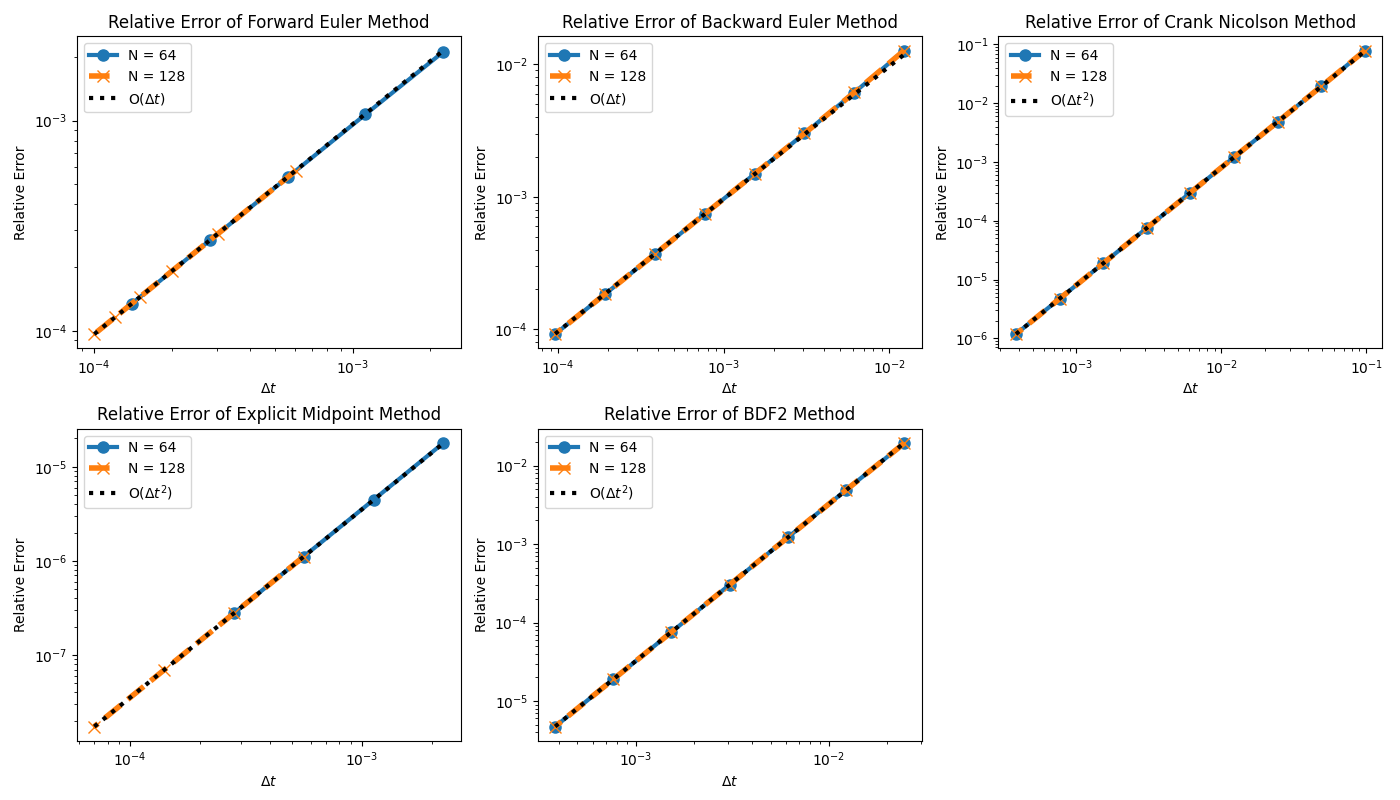
\includegraphics[width=1\textwidth]{figures/RelativeErrors.png}
    \caption{Relative error at $T = 2\pi$, Err $= \| \text{u}_\text{num} - \text{u}_\text{exact}\| / \|\text{u}_\text{exact}\|$, against time step $\Delta t$ on log-log plot, for each time-stepping method with $N = 64$ (blue circles) and $N =128$ (orange crosses). The black dotted lines in each log-log plot are reference slopes, $O(\Delta)$ for Forward and Backward Euler and $O(\Delta t^2)$ for Crank-Nicolson, Explicit Midpoint, and BDF2.}

    \label{fig:relerrors}
\end{figure}
    Every panel in Figure~\ref{fig:relerrors} shows that the data follows the reference slope which shows first-order convergence for Forward and Backward Euler and second-order convergence for Crank-Nicolson, Explicit Midpoint, and BDF2. The $\Delta t$ values for Forward Euler and Explicit Midpoint are restricted by the stability limit 
    \[\Delta t < \frac{1}{4} \Delta x^2 \implies                                  \frac{2N_x^2}{\pi} < N_t\]
    and the implicit methods have no stability restriction. Due to this each method had different time step sizes. For $N = 64$, the stability limit for the explicit methods means we must chose $N_t$ values such that 
    \[2608 < N_t\]
    which lead me to chose the values 
    \[N_t = \{2800, 5600, 11200, 22400, 44800\}\]
    For the implicit methods we don't have to worry about a restriction on $\Delta t$ for stability, but we do have to worry about accuracy. Accuracy for implicit methods depend on how small $\Delta t$ is relative to the system's timescale. To find good time stepping size I solved a coarse step $\Delta x$ then continued to refine it by halving the time stepping size with each implicit method and got \\
    \textbf{Backward Euler}
    \[N_t = \{2^9,2^{10},2^{11},2^{12},2^{13},2^{14},2^{15},2^{16},2^{17} \}\]
    \textbf{Crank Nicolson}
    \[N_t = \{2^5,2^6,2^7,2^8,2^9,2^{10},2^{11},2^{12},2^{13},2^{14},2^{15}\}\]
    \textbf{BDF2}
    \[N_t = \{2^8,2^9,2^{10},2^{11},2^{12},2^{13},2^{14},2^{15}\}\]
    For $N = 128$, the stability limit for the explicit methods means we must chose $N_t$ values such that 
    \[10431 < N_t\]
    which lead me to chose the values 
    \[N_t = \{10432, 20864, 31296, 41728, 52160, 62592\}\]
    I used the same $N_t$ values as $N =64$ for the implicit methods \\
    \textbf{Backward Euler}
    \[N_t = \{2^9,2^{10},2^{11},2^{12},2^{13},2^{14},2^{15},2^{16},2^{17} \}\]
    \textbf{Crank Nicolson}
    \[N_t = \{2^5,2^6,2^7,2^8,2^9,2^{10},2^{11},2^{12},2^{13},2^{14},2^{15}\}\]
    \textbf{BDF2}
    \[N_t = \{2^8,2^9,2^{10},2^{11},2^{12},2^{13},2^{14},2^{15}\}\]

    \section{Cost of Methods}
    To find the largest $\Delta t$ for the tolerance I created a function that I passed in a value of $N_t$ that had less than the tolerance and a $N_t$ value that was larger than the tolerance. For the explicit methods I passed in the minimum $N_t$ value for a stable approximation. \\
    The operations per step for the methods are as follows with the cheapest costs being highlighted
    \begin{center}
        \begin{tabular}{|c|c|c|c|} \hline
            Method & Multiplies & Solves & Factorization \\ \hline
            Forward Euler & 1 & 0 & none \\ \hline
            Backward Euler & 0 & 1 & 1 \\ \hline
            Crank-Nicolson & 1 & 1 & 1 \\ \hline
            Explicit Midpoint & & & none \\ \hline
            BDF2 & 0 & 1 & 1 per step (1 before every run) \\ \hline
        \end{tabular}
    \end{center}
    For $N = 64$, the cost are 
    \begin{center}
        \begin{tabular}{|c|c|c|c|c|} \hline
           tolerance & Method & Cost & Number of Steps \\ \hline
           $0.05$ & Forward Euler & 2608 & 50,125,760 \\ \hline
           $0.05$ & Backward Euler & 151 & 5,144,505\\ \hline
           \rowcolor{yellow!30} $0.05$ & Crank-Nicolson & 81 &  4,418,515 \\ \hline
           $0.05$ & Explicit Midpoint & 2608 & 100,251,520 \\ \hline
           $0.05$ & BDF2 & 156 & 5,314,852 \\ \hline
           $1\times10^{-3}$ & Forward Euler & 5997 & 115,262,340 \\ \hline
           $1\times10^{-3}$ & Backward Euler & 6078 & 207,074,847 \\ \hline
           \rowcolor{yellow!30} $1\times10^{-3}$ & Crank-Nicolson & 563 & 30,711,408 \\ \hline
           $1\times10^{-3}$ & Explicit Midpoint & 2608 & 100,251,520 \\ \hline
           $1\times10^{-3}$ & BDF2 & 1129 & 38,464,544 \\ \hline
           $5\times10^{-6}$ & Forward Euler & None & None \\ \hline
           $5\times10^{-6}$ & Backward Euler & 1207446 & 41,137,166,282 \\ \hline
           $5\times10^{-6}$ & Crank-Nicolson & 7955 & 433,941,831 \\ \hline
           \rowcolor{yellow!30} $5\times10^{-6}$ & Explicit Midpoint & 5288 & 203,270,720 \\ \hline
           $5\times10^{-6}$ & BDF2 & 15914 & 542,183,140 \\ \hline
        \end{tabular}
    \end{center}
    For $N = 128$, the cost are 
    \begin{center}
        \begin{tabular}{|c|c|c|c|c|} \hline
           tolerance & Method & Cost & Number of Steps \\ \hline
           $0.05$ & Forward Euler & 10431 & 854,507,520 \\  \hline
           $0.05$ & Backward Euler & 151 & 24,007,690 \\ \hline
           \rowcolor{yellow!30} $0.05$ & Crank-Nicolson & 81 & 19,513,817 \\ \hline
           $0.05$ & Explicit Midpoint & 10431 & 1,709,015,040 \\ \hline
           $0.05$ & BDF2 & 156 & 24,802,647 \\ \hline
           \rowcolor{yellow!30} $1\times10^{-3}$ & Forward Euler & 10431 & 50,125,760 \\ \hline
           $1\times10^{-3}$ & Backward Euler & 6078 & 966,349,289 \\ \hline
           $1\times10^{-3}$ & Crank-Nicolson & 563 & 135,633,077 \\ \hline
           $1\times10^{-3}$ & Explicit Midpoint & 10431 & 1,709,015,040 \\ \hline
           $1\times10^{-3}$ & BDF2 & 1129 & 179,501,208 \\ \hline
           $5\times10^{-6}$ & Forward Euler & None & None \\ \hline
           $5\times10^{-6}$ & Backward Euler & None & None \\ \hline
           $5\times10^{-6}$ & Crank-Nicolson & 7955 & 1,916,449,611 \\ \hline
           \rowcolor{yellow!30} $5\times10^{-6}$ & Explicit Midpoint & 10431 & 1,709,015,040 \\ \hline
           $5\times10^{-6}$ & BDF2 & 15913 & 2,530,028,997 \\ \hline
        \end{tabular}
    \end{center}
    Note that there is no number of steps that can get the Forward Euler relative error under $5 \times 10^{-6}$ with $N = 64, 128$ because the minimum $\Delta t$ has a relative larger then $5 \times 10^{-6}$. For the Backward Euler with tolerance of $5 \times 10^{-6}$ with $N = 128$ because the cost and time to calculate the numerical approximation is so high that it would most likely take an hour and we can see that it is no way near the method with the least cost with a higher tolerance with larger tolerances.
\end{document}